\documentclass[sigconf,nonacm]{acmart}

\setcopyright{none}
\settopmatter{printacmref=false}
\renewcommand\footnotetextcopyrightpermission[1]{}
\pagestyle{plain}

\usepackage{booktabs}
\usepackage{tabularx}
\usepackage{multirow}
\usepackage{amsmath}
\let\Bbbk\relax
\usepackage{amssymb}
\usepackage{tikz}
\usepackage{pgfplots}
\pgfplotsset{compat=1.18}
\usepackage{url}
\urlstyle{rm}

\usetikzlibrary{arrows.meta,positioning,calc,shapes.geometric,
                decorations.pathreplacing,patterns}

%% ── colour palette ────────────────────────────────────────────────────────
\definecolor{cred} {RGB}{200, 50, 50}
\definecolor{cora} {RGB}{210,110, 30}
\definecolor{cyel} {RGB}{200,175,  0}
\definecolor{cgrn} {RGB}{ 40,150, 70}
\definecolor{cblu} {RGB}{ 50,110,190}
\definecolor{cpur} {RGB}{130, 50,170}
\definecolor{cgry} {RGB}{100,100,100}

\begin{CCSXML}
<ccs2012>
  <concept>
    <concept_id>10002978.10003006.10003007</concept_id>
    <concept_desc>Security and privacy~Malware and its mitigation</concept_desc>
    <concept_significance>500</concept_significance>
  </concept>
  <concept>
    <concept_id>10002978.10003006</concept_id>
    <concept_desc>Security and privacy~Intrusion/anomaly detection and malware mitigation</concept_desc>
    <concept_significance>500</concept_significance>
  </concept>
  <concept>
    <concept_id>10002978.10003022</concept_id>
    <concept_desc>Security and privacy~Social engineering attacks</concept_desc>
    <concept_significance>300</concept_significance>
  </concept>
</ccs2012>
\end{CCSXML}

\ccsdesc[500]{Security and privacy~Malware and its mitigation}
\ccsdesc[300]{Security and privacy~Social engineering attacks}

\title{Ransomware in the Age of Social Engineering: Attack Vectors, High-Profile Breaches, and a Zero-Trust Defense Framework}

\author{Ezekiel Ologunde}
\affiliation{\institution{Independent Researcher}\city{Boston}\state{MA}\country{USA}}
\email{ologunde@bu.edu}

\begin{abstract}
Ransomware attacks have become a significant global threat targeting a broad spectrum
of Internet and mobile users, with critical cyber-physical systems particularly
vulnerable. This paper examines the anatomy of ransomware, its principal families
(CryptoWall, Locker, CryptoLocker, and WannaCry), and the pivotal role of social
engineering in enabling these attacks. We analyze three high-profile case studies---the
Colonial Pipeline shutdown (2021), the Kaseya VSA supply-chain incident (2021), and the
MGM Resorts breach (2020/2023)---documenting their attack vectors, financial impacts,
and recovery challenges. Our analysis demonstrates that human vulnerability, rather than
purely technical weakness, remains the primary attack surface exploited by ransomware
operators. We evaluate current defensive postures, identify critical gaps in existing
cyber threat training programs, and propose a multi-layered defense framework grounded
in Zero Trust architecture, multi-factor authentication, privileged access management,
and immutable offline backups. Finally, we identify priority future research directions,
including AI/ML-assisted detection, behavioral analytics, and the evolving threat
landscape posed by ransomware-as-a-service platforms.
\end{abstract}

\keywords{ransomware, social engineering, zero trust, malware, cyber-physical systems,
Colonial Pipeline, supply chain attack, multi-factor authentication, incident response}

\begin{document}
\hfuzz=5pt
\maketitle

%%────────────────────────────────────────────────────────────────────────────
\section{Introduction}
%%────────────────────────────────────────────────────────────────────────────

In today's cloud-driven digital environment, the term ``ransomware'' has become
all too familiar to security professionals. Ransomware refers to malicious software that
locks users out of their computer systems or denies access to services until a ransom is
paid. This form of cybercrime has evolved from isolated incidents into a lucrative
industrial-scale operation for criminal organizations worldwide~\cite{groot2023}.

One of the first documented ransomware attacks was the AIDS Trojan (PC Cyborg Virus),
released via floppy disk in 1989 by Joseph L.\ Popp, Ph.D., distributed to approximately
20,000 disks sent to AIDS researchers across more than 90 countries~\cite{baker2022}.
Victims were required to send \$189 to a P.O.\ box in Panama to restore access, despite
the malware relying on simple symmetric cryptography~\cite{baker2022}.

Today, stopping ransomware attacks has become dramatically more challenging because of
the lack of comprehensive understanding of how these attacks propagate. Two highly
notable recent examples are the attack on Colonial Pipeline---which briefly spiked U.S.
gas prices nationwide---and the record-setting \$44 million ransom payout by CNA
Financial~\cite{cleary2023,kerner2022}. As organizations invest in better security
technology, attackers have shifted focus to the weakest link in any security program:
the human end user. Social engineering is widely recognized as one of the most potent
weapons in an attacker's arsenal, because it is far easier to trick someone into
disclosing credentials than to brute-force cryptographic defenses.

This paper provides a comprehensive analysis of the ransomware threat landscape,
identifies the social engineering vectors that underpin most incidents, examines three
landmark case studies, and proposes a practical defense framework.

\subsection{Research Contributions}

\begin{itemize}
  \item Taxonomy of ransomware families and attack-chain stages with quantitative
        financial impact data
  \item Detailed analysis of Colonial Pipeline, Kaseya VSA, and MGM Resorts incidents
        identifying root-cause social engineering vectors
  \item Multi-layered defense framework integrating Zero Trust, MFA, PAM, and backup
        immutability
  \item Identification of gaps in existing cyber threat training programs and priority
        future research directions
\end{itemize}

%%────────────────────────────────────────────────────────────────────────────
\section{Ransomware: Taxonomy and Attack Chain}
%%────────────────────────────────────────────────────────────────────────────

\subsection{Definition and Etymology}

The word ``ransomware'' is a portmanteau of ``ransom'' and ``software.'' It refers to
malicious software that gains unauthorized access to files or systems and blocks user
access until a ransom is paid~\cite{groot2023,shea2023}. All files---or entire
devices---are held hostage via encryption until the demand is met.

\subsection{Principal Ransomware Families}

The two dominant ransomware families are \textbf{Crypto ransomware} and \textbf{Locker
ransomware}. Crypto variants (CryptoWall, CryptoLocker, WannaCry) encrypt files and
demand payment before providing the decryption key; victims' data is typically
threatened with permanent deletion if the ransom is not paid~\cite{ekta2021}.
Locker variants lock the operating system or device entirely, preventing the victim
from using the machine at all, independent of file encryption~\cite{savage2015}.
Figure~\ref{fig:families} maps the major ransomware families and their primary
characteristics.

\begin{figure}[h]
\centering
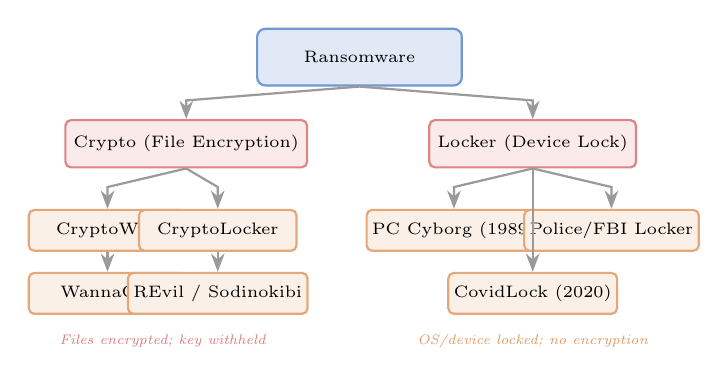
\begin{tikzpicture}[
  font=\fontsize{6.5pt}{8pt}\selectfont,
  >=Stealth,
  root/.style={rectangle, rounded corners=3pt, draw=cblu!70, thick,
               fill=cblu!15, minimum width=2.6cm, minimum height=0.72cm,
               text centered},
  fam/.style={rectangle, rounded corners=2pt, draw=cred!60, thick,
              fill=cred!10, minimum width=2.4cm, minimum height=0.60cm,
              text centered, inner sep=3pt},
  sub/.style={rectangle, rounded corners=2pt, draw=cora!60, thick,
              fill=cora!10, minimum width=2.0cm, minimum height=0.52cm,
              text centered, font=\fontsize{6pt}{7.5pt}\selectfont,
              inner sep=2pt},
  arr/.style={-{Stealth}, thick, cgry!65}
]
  \node[root] (R) at (0,0) {Ransomware};

  %% Two main branches
  \node[fam] (crypto) at (-2.2,-1.10) {Crypto (File Encryption)};
  \node[fam] (locker) at ( 2.2,-1.10) {Locker (Device Lock)};

  \draw[arr] (R.south) -- (-2.2,-0.55) -- (crypto.north);
  \draw[arr] (R.south) -- ( 2.2,-0.55) -- (locker.north);

  %% Crypto sub-families
  \node[sub] (cw)  at (-3.2,-2.20) {CryptoWall};
  \node[sub] (cl)  at (-1.8,-2.20) {CryptoLocker};
  \node[sub] (wc)  at (-3.2,-3.00) {WannaCry};
  \node[sub] (rv)  at (-1.8,-3.00) {REvil / Sodinokibi};

  \draw[arr] (crypto.south) -- (-3.2,-1.65) -- (cw.north);
  \draw[arr] (crypto.south) -- (-1.8,-1.65) -- (cl.north);
  \draw[arr] (cw.south) -- (wc.north);
  \draw[arr] (cl.south) -- (rv.north);

  %% Locker sub-families
  \node[sub] (pc)  at ( 1.2,-2.20) {PC Cyborg (1989)};
  \node[sub] (rev) at ( 3.2,-2.20) {Police/FBI Locker};
  \node[sub] (cvl) at ( 2.2,-3.00) {CovidLock (2020)};

  \draw[arr] (locker.south) -- (1.2,-1.65) -- (pc.north);
  \draw[arr] (locker.south) -- (3.2,-1.65) -- (rev.north);
  \draw[arr] (locker.south) -- (cvl.north);

  %% Impact labels
  \node[font=\fontsize{5.5pt}{7pt}\selectfont\itshape, text=cred!65]
    at (-2.5,-3.60) {Files encrypted; key withheld};
  \node[font=\fontsize{5.5pt}{7pt}\selectfont\itshape, text=cora!70]
    at ( 2.2,-3.60) {OS/device locked; no encryption};
\end{tikzpicture}
\caption{Ransomware family taxonomy. Crypto variants encrypt files and withhold
  decryption keys; Locker variants deny access to the operating system or device.}
\label{fig:families}
\end{figure}

\subsection{The Ransomware Kill Chain}

Figure~\ref{fig:killchain} illustrates the seven-stage ransomware attack chain from
initial compromise through ransom demand and recovery.

\begin{figure}[h]
\centering
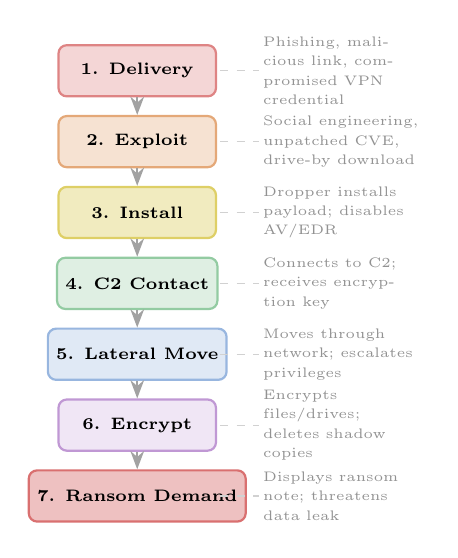
\begin{tikzpicture}[
  font=\fontsize{6.5pt}{8pt}\selectfont,
  >=Stealth,
  stg/.style={rectangle, rounded corners=3pt, draw, thick,
              minimum width=2.0cm, minimum height=0.65cm,
              text centered, inner sep=3pt},
  ann/.style={font=\fontsize{5.5pt}{7pt}\selectfont, text=cgry!70,
              align=left, text width=2.0cm},
  arr/.style={-{Stealth}, thick, cgry!60}
]
  %% Stages (left column, top to bottom)
  \node[stg, fill=cred!20, draw=cred!60]   (s1) at (0,  0.00) {\textbf{1. Delivery}};
  \node[stg, fill=cora!20, draw=cora!60]   (s2) at (0, -0.90) {\textbf{2. Exploit}};
  \node[stg, fill=cyel!25, draw=cyel!60]   (s3) at (0, -1.80) {\textbf{3. Install}};
  \node[stg, fill=cgrn!15, draw=cgrn!50]   (s4) at (0, -2.70) {\textbf{4. C2 Contact}};
  \node[stg, fill=cblu!15, draw=cblu!50]   (s5) at (0, -3.60) {\textbf{5. Lateral Move}};
  \node[stg, fill=cpur!12, draw=cpur!50]   (s6) at (0, -4.50) {\textbf{6. Encrypt}};
  \node[stg, fill=cred!30, draw=cred!70]   (s7) at (0, -5.40) {\textbf{7. Ransom Demand}};

  \foreach \a/\b in {s1/s2,s2/s3,s3/s4,s4/s5,s5/s6,s6/s7}
    \draw[arr] (\a)--(\b);

  %% Annotations (right column)
  \node[ann] at (2.6,  0.00) {Phishing, malicious link, compromised VPN credential};
  \node[ann] at (2.6, -0.90) {Social engineering, unpatched CVE, drive-by download};
  \node[ann] at (2.6, -1.80) {Dropper installs payload; disables AV/EDR};
  \node[ann] at (2.6, -2.70) {Connects to C2; receives encryption key};
  \node[ann] at (2.6, -3.60) {Moves through network; escalates privileges};
  \node[ann] at (2.6, -4.50) {Encrypts files/drives; deletes shadow copies};
  \node[ann] at (2.6, -5.40) {Displays ransom note; threatens data leak};

  %% Connecting dashes
  \foreach \y in {0.00,-0.90,-1.80,-2.70,-3.60,-4.50,-5.40}
    \draw[dashed, cgry!30] (1.05,\y) -- (1.55,\y);
\end{tikzpicture}
\caption{Seven-stage ransomware kill chain from initial delivery through ransom demand.
  Social engineering underlies the first two stages in the majority of incidents.}
\label{fig:killchain}
\end{figure}

Operating systems play an inevitable role in ransomware susceptibility. Devices running
Windows are most frequently targeted, though no operating system is immune---Apple iOS,
macOS, and Linux environments have all experienced ransomware
incidents~\cite{bhavsar2022,sultan2018}.

%%────────────────────────────────────────────────────────────────────────────
\section{Social Engineering as a Primary Attack Vector}
%%────────────────────────────────────────────────────────────────────────────

Social engineering is one of the most potent instruments in an attacker's arsenal
because it exploits human psychology rather than technical vulnerabilities. It is far
easier to deceive someone into surrendering credentials than to defeat cryptographic
defenses directly. Figure~\ref{fig:soceng} maps the key psychological attributes
exploited by social engineers and their corresponding attack techniques.

\begin{figure}[h]
\centering
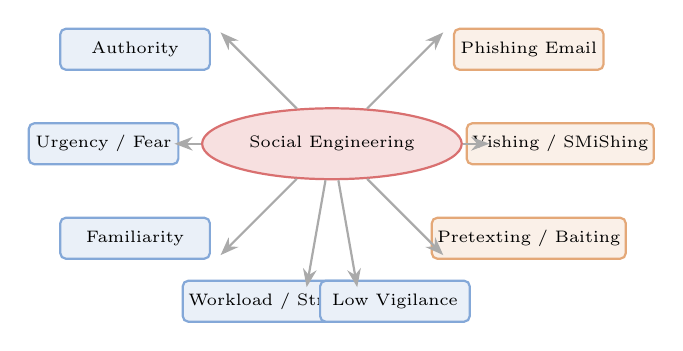
\begin{tikzpicture}[
  font=\fontsize{6.5pt}{8pt}\selectfont,
  >=Stealth,
  hub/.style={ellipse, draw=cred!70, thick, fill=cred!15,
              minimum width=2.2cm, minimum height=0.90cm, text centered},
  attr/.style={rectangle, rounded corners=2pt, draw=cblu!60, thick,
               fill=cblu!10, minimum width=1.90cm, minimum height=0.52cm,
               text centered, font=\fontsize{6pt}{7.5pt}\selectfont, inner sep=2pt},
  tech/.style={rectangle, rounded corners=2pt, draw=cora!60, thick,
               fill=cora!10, minimum width=1.90cm, minimum height=0.52cm,
               text centered, font=\fontsize{6pt}{7.5pt}\selectfont, inner sep=2pt},
  arr/.style={-{Stealth}, thick, cgry!55}
]
  \node[hub] (H) at (0,0) {Social Engineering};

  %% Psychological attributes — left semicircle
  \node[attr] at (-2.5,  1.2) {Authority};
  \node[attr] at (-2.9,  0.0) {Urgency / Fear};
  \node[attr] at (-2.5, -1.2) {Familiarity};

  %% Attack techniques — right semicircle
  \node[tech] at ( 2.5,  1.2) {Phishing Email};
  \node[tech] at ( 2.9,  0.0) {Vishing / SMiShing};
  \node[tech] at ( 2.5, -1.2) {Pretexting / Baiting};

  %% Enablers bottom
  \node[attr] at (-0.8, -2.0) {Workload / Stress};
  \node[attr] at ( 0.8, -2.0) {Low Vigilance};

  \foreach \a in {135,180,225}
    \draw[arr] (H) -- ++(\a:2.0);
  \foreach \a in {45,0,-45}
    \draw[arr] (H) -- ++(\a:2.0);
  \foreach \a in {-80,-100}
    \draw[arr] (H) -- ++(\a:1.85);
\end{tikzpicture}
\caption{Social engineering attack model: psychological attributes (blue) exploited
  by attackers through specific techniques (orange) targeting human susceptibility.}
\label{fig:soceng}
\end{figure}

Social engineering attributes that increase individual susceptibility include
personality traits, expertise level, cultural background, workload, stress, and
vigilance~\cite{aldawood2019}. Hackers weaponize these traits to penetrate security
perimeters and extract confidential credentials. Mitigation approaches include physical
security audits, policy enforcement, and awareness training---the last of which has
evolved from static video modules to immersive virtual simulations and real-world
phishing exercises~\cite{kontio2016}.

%%────────────────────────────────────────────────────────────────────────────
\section{High-Profile Case Studies}
%%────────────────────────────────────────────────────────────────────────────

\subsection{Colonial Pipeline (May 2021)}

On May 7, 2021, a ransomware attack struck the Colonial Pipeline Company, the primary
mover of gasoline, diesel, and jet fuel along the U.S.\ East Coast~\cite{beerman2023}.
Attackers from the DarkSide group discovered a dormant VPN account that lacked
multi-factor authentication~\cite{kerner2022}. Using compromised credentials, they
gained full network access, exfiltrated nearly 100\,GB of data, and deployed ransomware
that forced a six-day operational shutdown---the pipeline's first in 57 years. CEO
Joseph Blount authorized a payment of over \$4.4 million in Bitcoin to obtain the
decryption key. The resulting fuel shortage triggered panic buying, price spikes, and
a federal emergency declaration across multiple eastern states.

\textbf{Root cause:} Stale, credential-only VPN account with no MFA and no automated
access-review audit.

\subsection{Kaseya VSA Supply-Chain Attack (July 2021)}

In July 2021, the REvil ransomware group exploited a zero-day vulnerability in Kaseya
VSA, a widely-used remote monitoring and management platform. Within two hours---faster
than most network defense systems can respond---attackers compromised approximately
1,500 downstream managed service provider (MSP) customers in one of the largest
supply-chain ransomware incidents on record~\cite{leo2022}. The attackers demanded
\$70 million in cryptocurrency for a universal decryptor.

\textbf{Root cause:} Unpatched vendor software combined with trusted MSP supply-chain
access; no ``assume breach'' monitoring in downstream organizations.

\subsection{MGM Resorts International (2020 / 2023)}

In February 2020, personal information for 10.6 million MGM Resorts guests---including
names, phone numbers, email addresses, birth dates, and details of CEOs, celebrities,
and government employees---was posted on a hacking forum~\cite{moatsum2022}. In a
subsequent 2023 incident linked to social engineering of the IT help desk, MGM
experienced approximately \$100 million in total losses including earnings impact,
remediation costs, and legal fees~\cite{toulas2023}.

\textbf{Root cause:} Help-desk social engineering bypassing identity verification
procedures; insufficient privileged access controls and session monitoring.

\subsection{CovidLock (2020)}

During the COVID-19 pandemic, an Android application purporting to display heat map
statistics for COVID-19 distributed a locker payload dubbed
CovidLock~\cite{saeed2020}. Upon installation, it locked contacts, photos, videos, and
social media access, demanding Bitcoin ransom under threat of public data release.
This incident illustrates how attackers weaponize public health emergencies to engineer
urgency-driven installation.

Figure~\ref{fig:impacts} compares the financial and operational impact of each case
study.

\begin{figure}[h]
\centering
\resizebox{\columnwidth}{!}{%
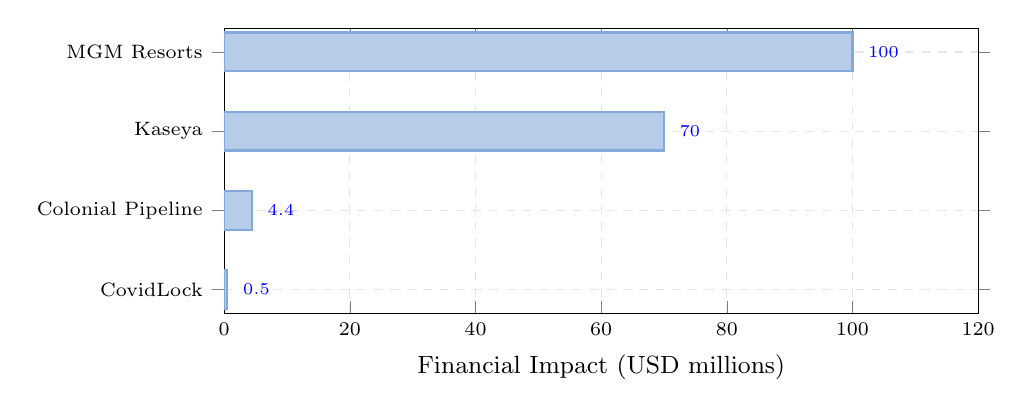
\begin{tikzpicture}
\begin{axis}[
  xbar,
  width=0.92\columnwidth, height=5.2cm,
  xlabel={Financial Impact (USD millions)},
  xlabel style={font=\small},
  ytick={1,2,3,4},
  yticklabels={CovidLock, Colonial Pipeline, Kaseya, MGM Resorts},
  yticklabel style={font=\scriptsize},
  tick label style={font=\scriptsize},
  xmin=0, xmax=120,
  grid=major, grid style={dashed, gray!20},
  bar width=14pt,
  nodes near coords,
  nodes near coords style={font=\fontsize{6pt}{7.5pt}\selectfont, xshift=2pt},
  every axis plot post/.style={fill=cblu!35, draw=cblu!60, thick}
]
  \addplot coordinates {(0.5,1) (4.4,2) (70,3) (100,4)};
\end{axis}
\end{tikzpicture}
}%
\caption{Financial impact comparison across the four case studies (USD millions).
  Kaseya and MGM illustrate the escalating scale of ransomware financial demands.}
\label{fig:impacts}
\end{figure}

%%────────────────────────────────────────────────────────────────────────────
\section{Defense Framework}
%%────────────────────────────────────────────────────────────────────────────

Based on lessons drawn from the case studies and existing literature, we propose a
five-layer defense framework. Figure~\ref{fig:defense} illustrates the layered
architecture.

\begin{figure}[h]
\centering
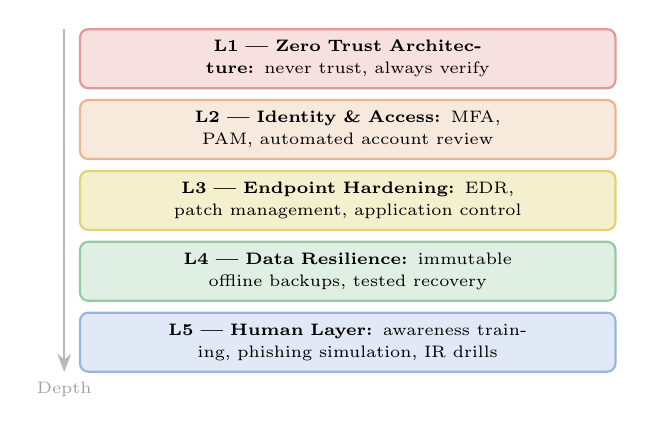
\begin{tikzpicture}[
  font=\fontsize{6.5pt}{8pt}\selectfont,
  >=Stealth,
  lyr/.style={rectangle, rounded corners=3pt, draw, thick,
              minimum width=6.8cm, minimum height=0.75cm,
              text centered, text width=6.5cm, inner sep=3pt}
]
  \node[lyr, fill=cred!15, draw=cred!50]  (l1) at (0, 0.00)
    {\textbf{L1 — Zero Trust Architecture:} never trust, always verify};
  \node[lyr, fill=cora!15, draw=cora!50]  (l2) at (0,-0.90)
    {\textbf{L2 — Identity \& Access:} MFA, PAM, automated account review};
  \node[lyr, fill=cyel!20, draw=cyel!55]  (l3) at (0,-1.80)
    {\textbf{L3 — Endpoint Hardening:} EDR, patch management, application control};
  \node[lyr, fill=cgrn!15, draw=cgrn!50]  (l4) at (0,-2.70)
    {\textbf{L4 — Data Resilience:} immutable offline backups, tested recovery};
  \node[lyr, fill=cblu!15, draw=cblu!50]  (l5) at (0,-3.60)
    {\textbf{L5 — Human Layer:} awareness training, phishing simulation, IR drills};

  \draw[-{Stealth}, thick, cgry!45] (-3.6,0.38) -- (-3.6,-3.98)
    node[below, font=\fontsize{6pt}{7.5pt}\selectfont, text=cgry!60] {Depth};
\end{tikzpicture}
\caption{Five-layer ransomware defense framework. Zero Trust at the perimeter is
  necessary but insufficient without strong identity controls and a resilient human
  layer.}
\label{fig:defense}
\end{figure}

\subsection{Layer 1 — Zero Trust Architecture}

Zero Trust posits that no packet, user, or device is inherently trusted, whether inside
or outside the organizational perimeter~\cite{saeed2020}. Every access request must be
authenticated, authorized, and continuously validated. Key principles include:
least-privilege access to only the hosts, ports, and applications required for a given
role; micro-segmentation to limit lateral movement; and continuous session monitoring
with automatic termination on anomaly detection.

\subsection{Layer 2 — Identity and Access Management}

The Colonial Pipeline incident illustrates the catastrophic consequence of a single
dormant, credential-only account. Mitigation requires:
\begin{itemize}
  \item \textbf{Multi-Factor Authentication (MFA):} requiring two or more authorization
        factors before granting access to any network service, particularly VPN and
        remote desktop interfaces~\cite{saeed2020}
  \item \textbf{Privileged Access Management (PAM):} just-in-time access provisioning
        with time-limited sessions for administrative accounts
  \item \textbf{Automated Account Review:} continuous audit flagging dormant or
        orphaned accounts for prompt deactivation
\end{itemize}

\subsection{Layer 3 — Endpoint Hardening and Patch Management}

Windows environments are disproportionately targeted, yet no operating system is
immune~\cite{sultan2018}. Essential controls include:
\begin{itemize}
  \item Endpoint Detection and Response (EDR) with behavioral analysis capable of
        identifying ransomware staging activities (shadow copy deletion, mass file
        renaming)
  \item Systematic vulnerability management prioritizing internet-facing systems and
        software with known exploit code in the wild (e.g., Kaseya CVE)
  \item Application allowlisting to prevent unauthorized executable launches
\end{itemize}

\subsection{Layer 4 — Data Resilience and Backup Strategy}

Regular backups can significantly reduce the operational impact of ransomware, limiting
harm to data created since the last backup point~\cite{cleary2023}. Critical
implementation considerations include:
\begin{itemize}
  \item \textbf{Immutable offline backups:} stored in air-gapped or write-once media
        inaccessible to ransomware payloads
  \item \textbf{Backup integrity validation:} scanning backup copies for malware before
        any restoration procedure
  \item \textbf{Recovery testing:} regular restoration drills verifying actual
        recoverability under time pressure
\end{itemize}

\subsection{Layer 5 — Security Awareness and Training}

Research consistently identifies human error as the primary entry point for ransomware.
Effective training programs have evolved from static video modules toward immersive
formats~\cite{kontio2016}:
\begin{itemize}
  \item Simulated phishing campaigns with immediate, personalized feedback loops
  \item Tabletop incident response exercises simulating ransomware scenarios
  \item Role-specific training tailored to the social engineering vectors most relevant
        to each job function (e.g., help-desk staff for voice phishing)
\end{itemize}

The finding from our case study analysis suggests that awareness training should be
prioritized \emph{before} deployment of new technical protection tools, as even
state-of-the-art technology cannot compensate for an untrained human layer.

%%────────────────────────────────────────────────────────────────────────────
\section{Zero Trust in Practice: A Decision Model}
%%────────────────────────────────────────────────────────────────────────────

Figure~\ref{fig:zt_decision} presents a simplified decision model for Zero Trust access
evaluation, showing how each access request is evaluated continuously rather than
implicitly trusted after initial authentication.

\begin{figure}[h]
\centering
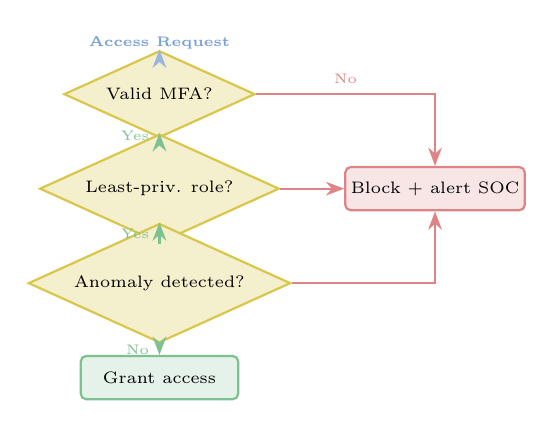
\begin{tikzpicture}[
  font=\fontsize{6.5pt}{8pt}\selectfont,
  >=Stealth,
  dec/.style={diamond, draw=cyel!70, thick, fill=cyel!20, aspect=2.2,
              minimum width=2.2cm, minimum height=0.70cm,
              text centered, font=\fontsize{6pt}{7.5pt}\selectfont},
  act/.style={rectangle, rounded corners=2pt, draw=cgrn!60, thick,
              fill=cgrn!12, minimum width=2.0cm, minimum height=0.55cm,
              text centered, font=\fontsize{6pt}{7.5pt}\selectfont, inner sep=2pt},
  blk/.style={rectangle, rounded corners=2pt, draw=cred!60, thick,
              fill=cred!12, minimum width=2.0cm, minimum height=0.55cm,
              text centered, font=\fontsize{6pt}{7.5pt}\selectfont, inner sep=2pt},
  arr/.style={-{Stealth}, thick}
]
  \node[dec] (d1) at (0,  0.00) {Valid MFA?};
  \node[dec] (d2) at (0, -1.20) {Least-priv. role?};
  \node[dec] (d3) at (0, -2.40) {Anomaly detected?};
  \node[act] (ok) at (0, -3.60) {Grant access};
  \node[blk] (bk) at (3.5,-1.20) {Block + alert SOC};

  \draw[arr, cgrn!60] (d1.south)--node[left,font=\fontsize{5.5pt}{7pt}\selectfont]{Yes}(d2.north);
  \draw[arr, cred!60] (d1.east)--node[above,font=\fontsize{5.5pt}{7pt}\selectfont]{No}(3.5,0) -- (bk.north);
  \draw[arr, cgrn!60] (d2.south)--node[left,font=\fontsize{5.5pt}{7pt}\selectfont]{Yes}(d3.north);
  \draw[arr, cred!60] (d2.east)--(bk.west);
  \draw[arr, cgrn!60] (d3.south)--node[left,font=\fontsize{5.5pt}{7pt}\selectfont]{No}(ok.north);
  \draw[arr, cred!60] (d3.east)--(3.5,-2.40) -- (bk.south);

  \node[font=\fontsize{5.5pt}{7pt}\selectfont\bfseries, text=cblu!65]
    at (0, 0.65) {Access Request};
  \draw[-{Stealth}, cblu!50, thick] (0,0.45)--(d1.north);
\end{tikzpicture}
\caption{Zero Trust continuous access evaluation model: every request is verified
  against MFA, least-privilege role constraints, and real-time anomaly detection before
  access is granted.}
\label{fig:zt_decision}
\end{figure}

%%────────────────────────────────────────────────────────────────────────────
\section{Analysis and Discussion}
%%────────────────────────────────────────────────────────────────────────────

\subsection{The Human-Technology Imbalance}

Across all four case studies, the initial compromise was enabled by human factors rather
than by defeating hardened technical defenses. The Colonial Pipeline attacker required
only a dormant VPN credential. The Kaseya attack exploited a vendor's unpatched
software---but the downstream impact was amplified by unconditional trust in MSP access.
MGM's breach began with a phone call to the help desk. This pattern underscores that
technology investment alone is insufficient without commensurate investment in human
resilience.

\subsection{The Ransom Payment Dilemma}

Paying or refusing to pay the ransom presents a complex moral, ethical, and pragmatic
dilemma. Payment does not guarantee data recovery, emboldens future attacks, and may
violate OFAC sanctions when payments reach sanctioned entities. Conversely, refusal may
result in permanent data loss and public release of exfiltrated information. This
dilemma reinforces the value of robust backup strategies that eliminate the necessity
of payment as a recovery option.

\subsection{Training Program Gaps}

Current cyber threat training programs provide fundamental knowledge of cybersecurity
concepts but often fail to keep pace with the rapidly evolving ransomware landscape.
Specific gaps identified include: insufficient coverage of voice phishing (vishing) and
help-desk social engineering; limited scenario diversity that does not reflect
attacker-specific pretexting for targeted roles; and inadequate post-incident
debriefing that could convert near-misses into learning opportunities.

%%────────────────────────────────────────────────────────────────────────────
\section{Future Research Directions}
%%────────────────────────────────────────────────────────────────────────────

\subsection{AI and Machine Learning for Ransomware Detection}

Information security professionals should explore how AI and ML can be leveraged to
detect ransomware earlier in the kill chain. Behavioral analytics can identify
ransomware-precursor activities---anomalous file renaming patterns, shadow copy
enumeration, and unusual network beaconing---before encryption begins. Large language
models offer potential for automated threat intelligence extraction and real-time
phishing detection.

\subsection{Ransomware-as-a-Service (RaaS) Platform Analysis}

The proliferation of RaaS platforms has democratized ransomware deployment, enabling
low-skill affiliates to launch sophisticated attacks. Research should map the economic
structure of RaaS ecosystems, identify leverage points for disruption (cryptocurrency
mixers, forum takedowns, affiliate recruitment), and develop threat intelligence
frameworks tailored to RaaS campaign attribution.

\subsection{Quantifying Social Engineering Risk}

There is a significant gap in quantitative models for predicting individual and
organizational susceptibility to social engineering. Factors including cognitive load,
organizational culture, industry sector, and prior training exposure warrant systematic
study to inform evidence-based training program design.

\subsection{Supply Chain Security}

The Kaseya incident demonstrates that third-party software vendors represent a force
multiplier for ransomware operators. Research should develop standardized security
assessment frameworks for software supply chains, including software bills of materials
(SBOMs), cryptographic build attestation, and contractual security requirements for
MSP relationships.

\subsection{Academia-Industry Collaboration}

A synergistic approach incorporating both academic and private-sector perspectives can
yield comprehensive insights and practical solutions. Joint studies can serve as
crucibles of innovation, fostering voluntary industry-wide best practices and
establishing reliable, resilient networks.

%%────────────────────────────────────────────────────────────────────────────
\section{Conclusion}
%%────────────────────────────────────────────────────────────────────────────

Every aspect of modern organizational life is intertwined with technology, making secure
operations an existential imperative. This paper has examined the anatomy of ransomware,
the centrality of social engineering as an attack enabler, and the lessons embedded in
four high-profile incidents. The findings converge on a clear conclusion: organizations
must treat the human layer as a primary attack surface deserving of investment
commensurate with that devoted to technical controls.

The five-layer defense framework proposed here---Zero Trust architecture, hardened
identity management, endpoint protection, data resilience, and human awareness
training---provides a structured approach to reducing ransomware risk without relying
on any single technology as a silver bullet. The research further suggests that training
and awareness programs should be \emph{prioritized before} new technical tools, as
untrained personnel will inevitably circumvent even well-designed controls.

Looking forward, AI/ML-assisted behavioral detection, robust supply chain security
standards, and quantitative social engineering risk models represent the most promising
avenues for advancing the field. Fostering collaboration between academia and private
industry will be essential to stay ahead of ransomware operators, whose own capabilities
continue to evolve through the very service platforms and affiliate networks that make
them so formidable.

\begin{acks}
The author acknowledges the contributions of the cybersecurity research community
and the incident analysis teams whose post-breach disclosures form the empirical
foundation of this study.
\end{acks}

\sloppy
\bibliographystyle{ACM-Reference-Format}
\begin{thebibliography}{20}

\bibitem{aldawood2019}
H.~Aldawood and G.~Skinner. 2019. An Academic Review of Current Industrial and
Commercial Social Engineering Awareness Training. In \textit{Proc.\ 3rd Int.\ Conf.\ on
Cryptography, Security and Privacy}. 110--115.

\bibitem{baker2022}
K.~Baker. 2022. \textit{History of Ransomware}. CrowdStrike.
\url{https://www.crowdstrike.com/cybersecurity-101/ransomware/history-of-ransomware/}

\bibitem{beerman2023}
J.~Beerman and D.~Baca. 2023. A Review of Colonial Pipeline Ransomware Attack. In
\textit{Proc.\ IEEE/ACM 23rd Int.\ Symp.\ on Cluster, Cloud and Internet Computing
Workshops (CCGridW)}. IEEE, 9--16.

\bibitem{bhavsar2022}
K.~C.~Bhavsar, N.~P.~Patel, and S.~C.~Vasoya. 2022. A Systematic Literature Review on
Ransomware Attacks. \textit{arXiv preprint} (cs.CY) (2022).

\bibitem{cleary2023}
Q.~Cleary. 2023. \textit{The Devastating Impact of Ransomware Attacks on Small
Businesses}. University of Maryland Law School.
\url{https://www.law.umaryland.edu/content/articles/name-659577-en.html}

\bibitem{ekta2021}
U.~B.~Ekta. 2021. A Review on Ransomware Attack. In \textit{Proc.\ 2021 2nd Int.\
Conf.\ on Secure Cyber Computing and Communications (ICSCCC)}. IEEE.

\bibitem{groot2023}
J.~D.~Groot. 2023. \textit{What Is Ransomware?} Digital Guardian.
\url{https://www.digitalguardian.com/blog/what-data-encryption}

\bibitem{kerner2022}
S.~M.~Kerner. 2022. \textit{Colonial Pipeline Hack Explained: Everything You Need to
Know}. TechTarget. \url{https://www.techtarget.com/whatis/feature/Colonial-Pipeline-hack-explained-Everything-you-need-to-know}

\bibitem{kontio2016}
M.~Kontio. 2016. Social Engineering 101. (2016).

\bibitem{leo2022}
P.~I.~Leo. 2022. The Ransomware Dilemma. \textit{MIT Sloan Management Review} (2022),
13--15.

\bibitem{moatsum2022}
Moatsum, Abiodun, Oludare, and Murad. 2022. A Deeper Look into Cybersecurity Issues in
the Wake of Covid-19. \textit{J.\ King Saud University --- Computer and Information
Sciences} (2022), 8176--8206.

\bibitem{montan2021}
R.~Montan\~{a} and A.~Ans. 2021. Social Engineering Attacks and Defences. In
\textit{Seeking Foundations for the Science of Cyber Security}. 263--267.

\bibitem{saeed2020}
M.~A.~Saeed. 2020. Malware in Computer Systems: Problems and Solutions. \textit{J.\
Informatics for Development} (2020), 1--8.

\bibitem{savage2015}
K.~Savage, P.~Coogan, and H.~Lau. 2015. The Evolution of Ransomware. Symantec Security
Response.

\bibitem{shea2023}
S.~Shea. 2023. \textit{What is Ransomware?} TechTarget.
\url{https://www.techtarget.com/searchsecurity/definition/ransomware}

\bibitem{sultan2018}
H.~Sultan and A.~Khan. 2018. A Survey on Ransomware: Evolution, Growth, and Impact.
\textit{Int.\ J.\ Adv.\ Res.\ Comput.\ Sci.} 10 (2018).

\bibitem{toulas2023}
B.~Toulas. 2023. \textit{MGM Resorts Ransomware Attack Led to \$100 Million Loss, Data
Theft}. Bleeping Computer.
\url{https://www.bleepingcomputer.com/news/security/mgm-resorts-ransomware-attack-led-to-100-million-loss-data-theft/}

\end{thebibliography}

\end{document}
